%%% Appendix.tex --- 
%% 
%% Filename: Appendix.tex
%% Author: Jacob Ringfjord & Max Wilén
%%% Code:


\begin{appendices}
\chapter{Appendix}
\newpage

\begin{figure}[H]
    \centering
    \lstinputlisting[language=json]{code_blocks/ghidriff_json_output.json}
    \caption{Ghidriff output in JSON format from Signal v7.34.2 and v7.35.0}
    \label{fig:ghidriff_json_output_A}
\end{figure}

\begin{figure}[H]
    \centering
    \lstinputlisting[language=json]{code_blocks/ghidriff_json_output_2.json}
    \caption{Ghidriff output in JSON format from Signal v7.34.2 and v7.35.0}
    \label{fig:ghidriff_json_output_B}
\end{figure}

\begin{figure}[H]
    \centering
    \lstinputlisting[language=json]{code_blocks/ghidriff_json_output_3.json}
    \caption{Ghidriff output in JSON format from Signal v7.34.2 and v7.35.0}
    \label{fig:ghidriff_json_output_C}
\end{figure}

\begin{comment}
\begin{figure}[H]
    \centering
    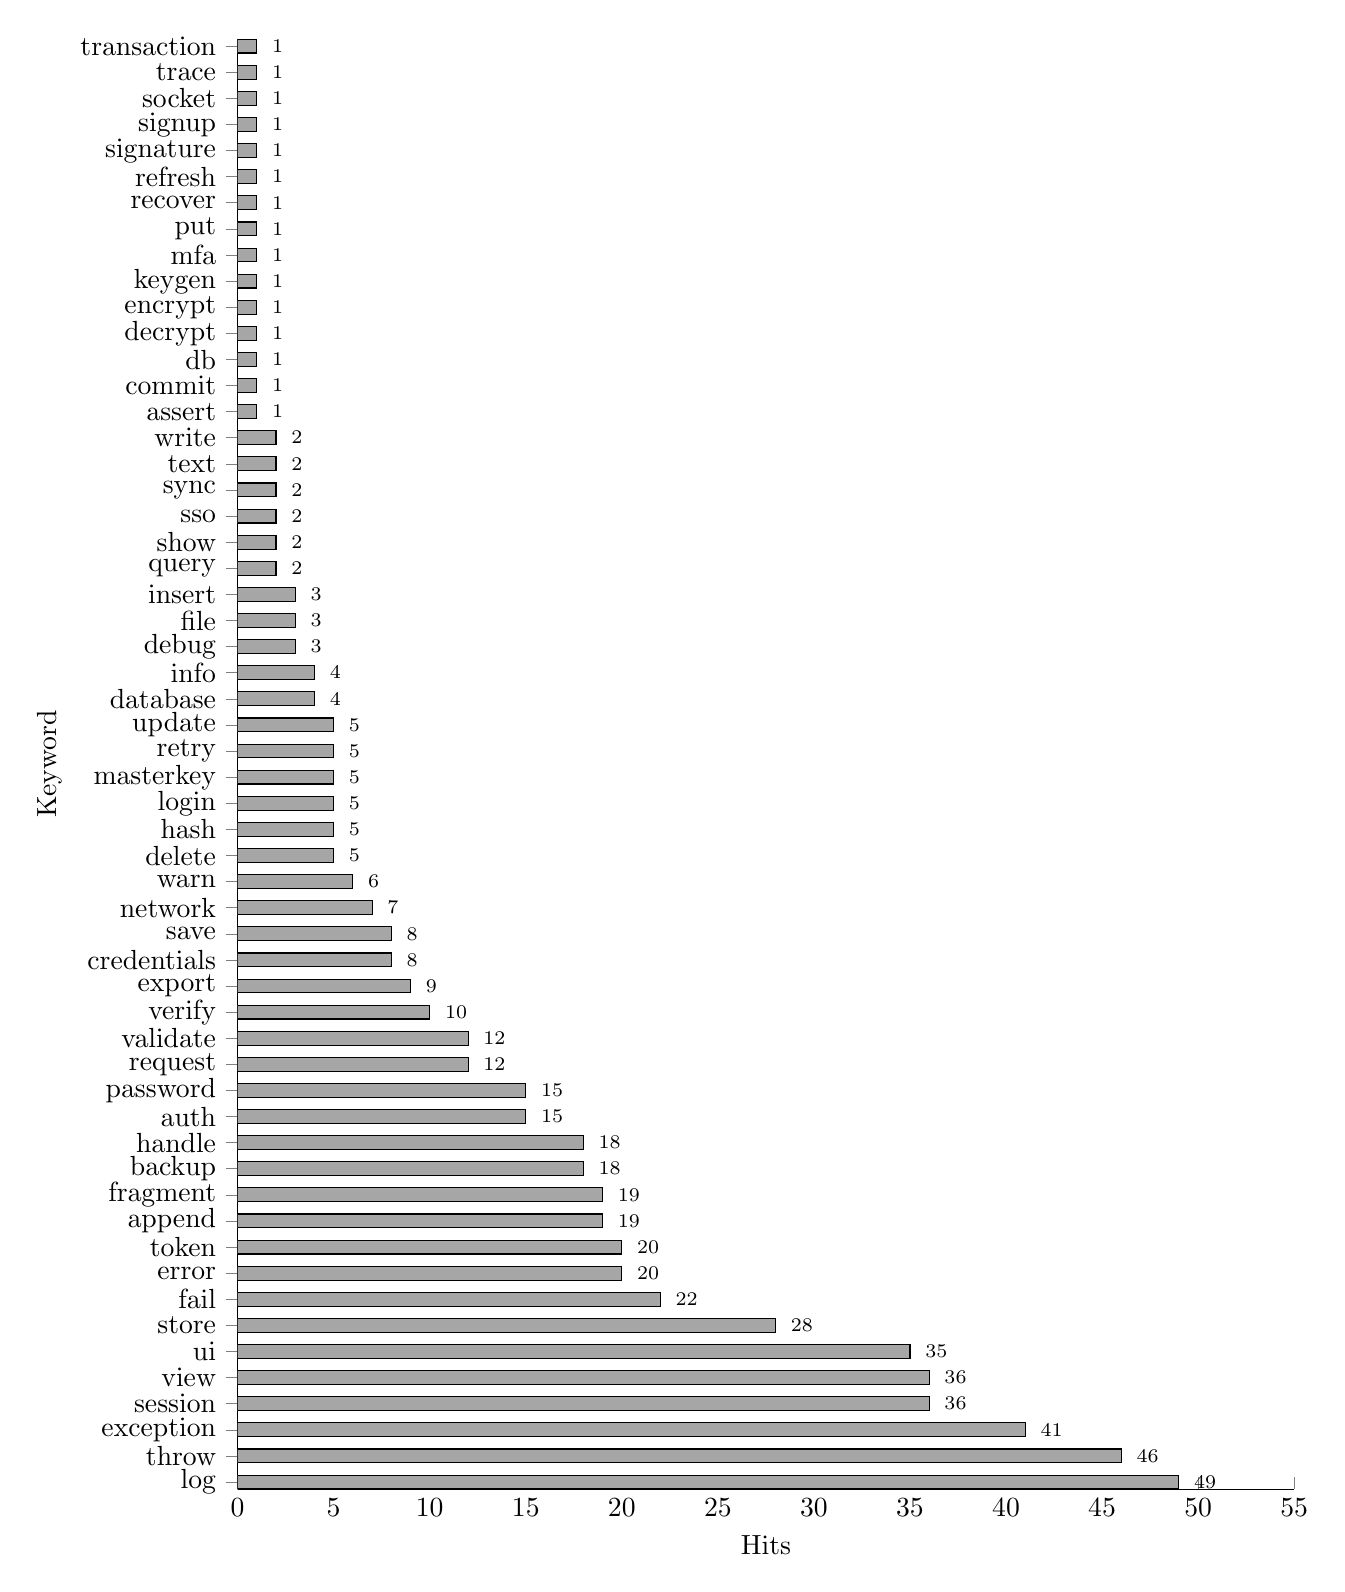
\begin{tikzpicture}
      \begin{axis}[
        width=15cm,
        height=20cm,
        xbar,
        bar width=5pt,
        symbolic y coords={
            log,throw,exception,session,view,ui,store,fail,error,token,
            append,fragment,backup,handle,auth,password,request,validate,
            verify,export,credentials,save,network,warn,delete,hash,login,
            masterkey,retry,update,database,info,debug,file,insert,query,
            show,sso,sync,text,write,assert,commit,db,decrypt,encrypt,
            keygen,mfa,put,recover,refresh,signature,signup,socket,trace,
            transaction},
        ytick=data,
        tick label style={font=\normalsize},
        enlarge y limits=0.005,
        xlabel={Hits},
        ylabel={Keyword},
        xmin=0, xmax=55,
        nodes near coords,
        every node near coord/.append style={font=\scriptsize,xshift=2pt},
        axis x line*=bottom,
        axis y line*=left
      ]
        \addplot[xbar,fill=gray!70] coordinates {
          (49,log) (46,throw) (41,exception) (36,session) (36,view)
          (35,ui) (28,store) (22,fail) (20,error) (20,token)
          (19,append) (19,fragment) (18,backup) (18,handle)
          (15,auth) (15,password) (12,request) (12,validate)
          (10,verify) (9,export) (8,credentials) (8,save)
          (7,network) (6,warn) (5,delete) (5,hash) (5,login)
          (5,masterkey) (5,retry) (5,update) (4,database)
          (4,info) (3,debug) (3,file) (3,insert) (2,query)
          (2,show) (2,sso) (2,sync) (2,text) (2,write)
          (1,assert) (1,commit) (1,db) (1,decrypt) (1,encrypt)
          (1,keygen) (1,mfa) (1,put) (1,recover) (1,refresh)
          (1,signature) (1,signup) (1,socket) (1,trace)
          (1,transaction)
        };
      \end{axis}
    \end{tikzpicture}
    \caption{All keyword hits generating categorizations in version diff A}
    \label{fig:commonly_used_words_A_full_sorted}
\end{figure}


\begin{figure}[H]
    \centering
    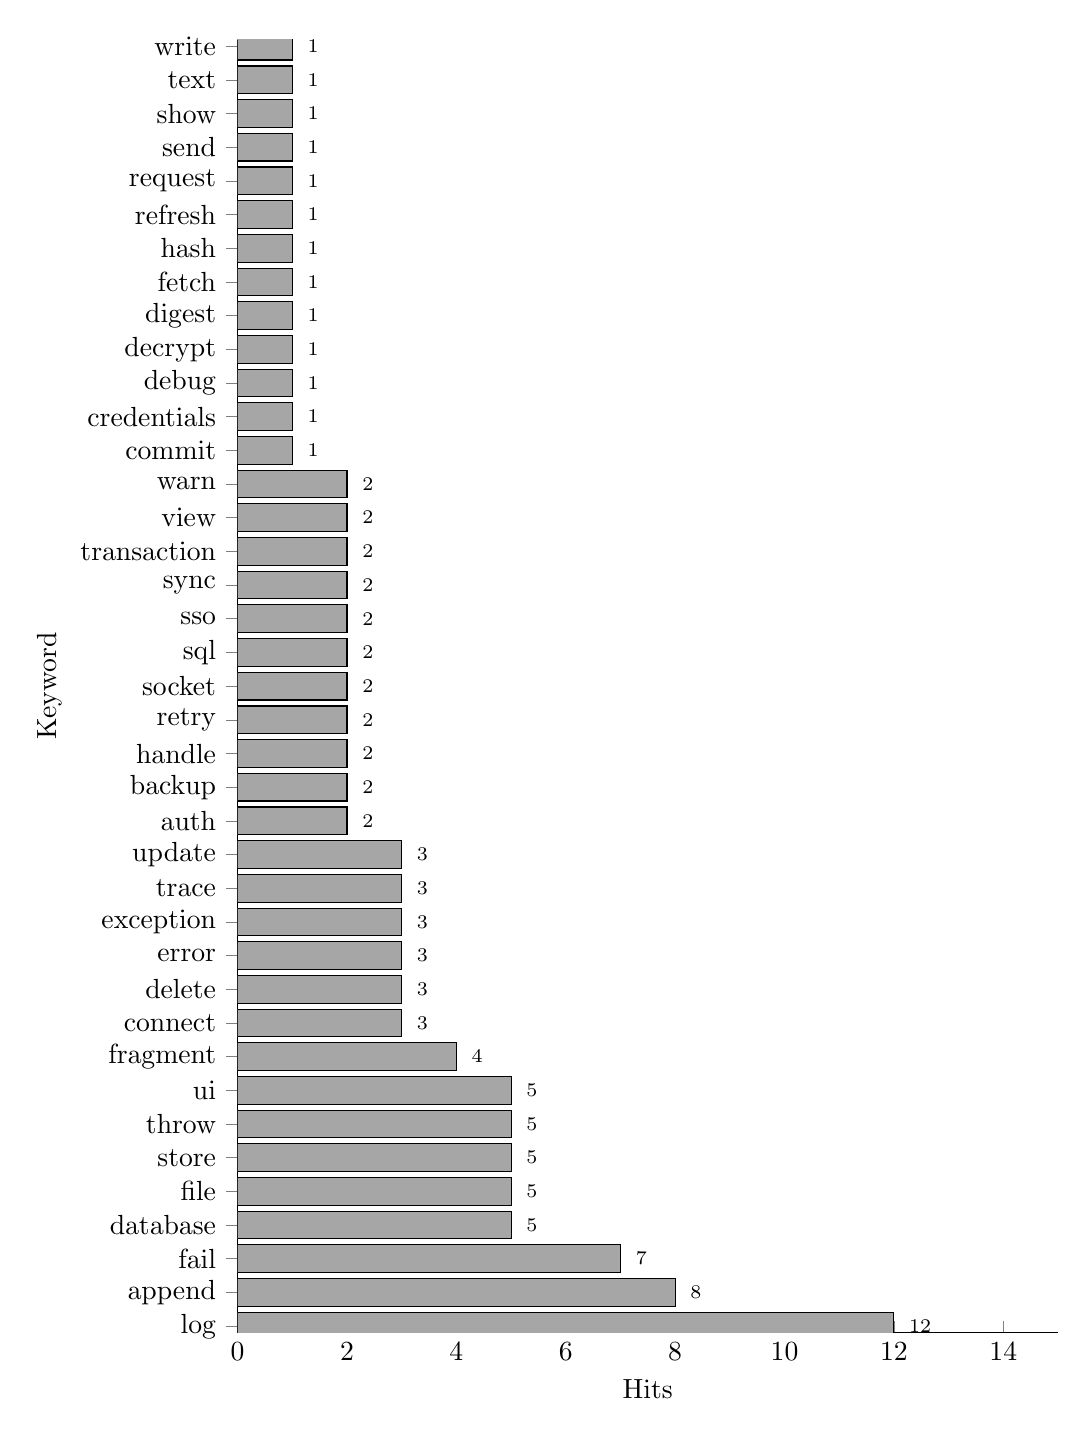
\begin{tikzpicture}
      \begin{axis}[
        width=12cm,
        height=18cm,
        xbar,
        bar width=10pt,
        symbolic y coords={
            log,append,fail,database,file,store,throw,ui,fragment,connect,
            delete,error,exception,trace,update,auth,backup,handle,retry,
            socket,sql,sso,sync,transaction,view,warn,commit,credentials,
            debug,decrypt,digest,fetch,hash,refresh,request,send,show,text,
            write},
        ytick=data,
        tick label style={font=\normalsize},
        enlarge y limits=0.005,
        xlabel={Hits},
        ylabel={Keyword},
        xmin=0, xmax=15,
        nodes near coords,
        every node near coord/.append style={font=\scriptsize,xshift=2pt},
        axis x line*=bottom,
        axis y line*=left
      ]
        \addplot[xbar,fill=gray!70] coordinates {
          (12,log) (8,append) (7,fail) (5,database) (5,file) (5,store)
          (5,throw) (5,ui) (4,fragment) (3,connect) (3,delete) (3,error)
          (3,exception) (3,trace) (3,update) (2,auth) (2,backup) (2,handle)
          (2,retry) (2,socket) (2,sql) (2,sso) (2,sync) (2,transaction)
          (2,view) (2,warn) (1,commit) (1,credentials) (1,debug) (1,decrypt)
          (1,digest) (1,fetch) (1,hash) (1,refresh) (1,request) (1,send)
          (1,show) (1,text) (1,write)
        };
      \end{axis}
    \end{tikzpicture}
    \caption{All keywords hits generating categorizations in version diff B}
    \label{fig:commonly_used_words_B_full_rotated}
\end{figure}

\begin{figure}[H]
    \centering
    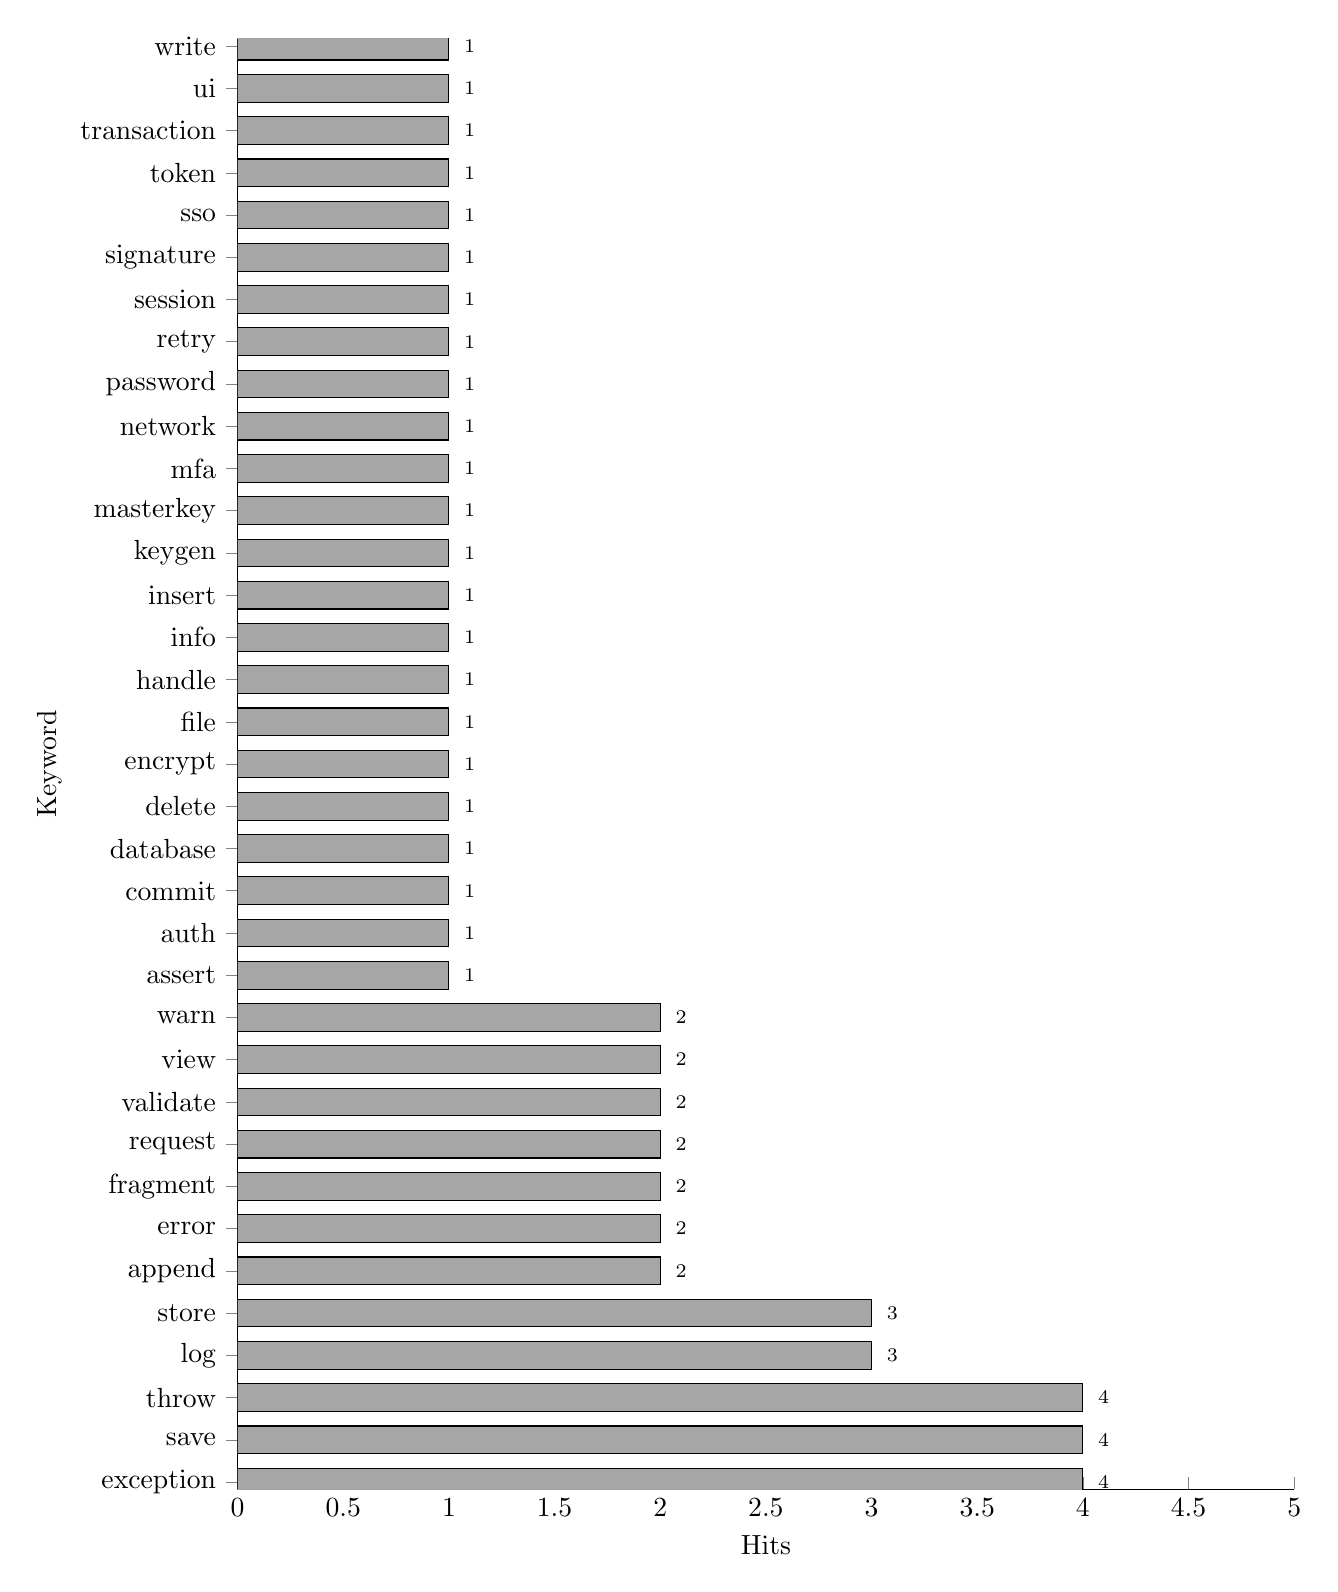
\begin{tikzpicture}
      \begin{axis}[
        width=15cm,
        height=20cm,
        xbar,
        bar width=10pt,
        symbolic y coords={
          exception,save,throw,log,store,append,error,fragment,request,validate,
          view,warn,assert,auth,commit,database,delete,encrypt,file,handle,info,
          insert,keygen,masterkey,mfa,network,password,retry,session,signature,
          sso,token,transaction,ui,write},
        ytick=data,
        tick label style={font=\normalsize},
        enlarge y limits=0.005,
        xlabel={Hits},
        ylabel={Keyword},
        xmin=0, xmax=5,
        nodes near coords,
        every node near coord/.append style={font=\scriptsize,xshift=2pt},
        axis x line*=bottom,
        axis y line*=left
      ]
        \addplot[xbar,fill=gray!70] coordinates {
          (4,exception) (4,save) (4,throw)
          (3,log) (3,store)
          (2,append) (2,error) (2,fragment) (2,request) (2,validate)
          (2,view) (2,warn)
          (1,assert) (1,auth) (1,commit) (1,database) (1,delete)
          (1,encrypt) (1,file) (1,handle) (1,info) (1,insert) (1,keygen)
          (1,masterkey) (1,mfa) (1,network) (1,password) (1,retry)
          (1,session) (1,signature) (1,sso) (1,token) (1,transaction)
          (1,ui) (1,write)
        };
      \end{axis}
    \end{tikzpicture}
    \caption{All keywords resulting in incorrect categorization for version diff A}
    \label{fig:keyword_incorrect_trigger_A_full_rotated}
\end{figure}
\end{comment}

\newpage
\begin{figure}
    \centering
    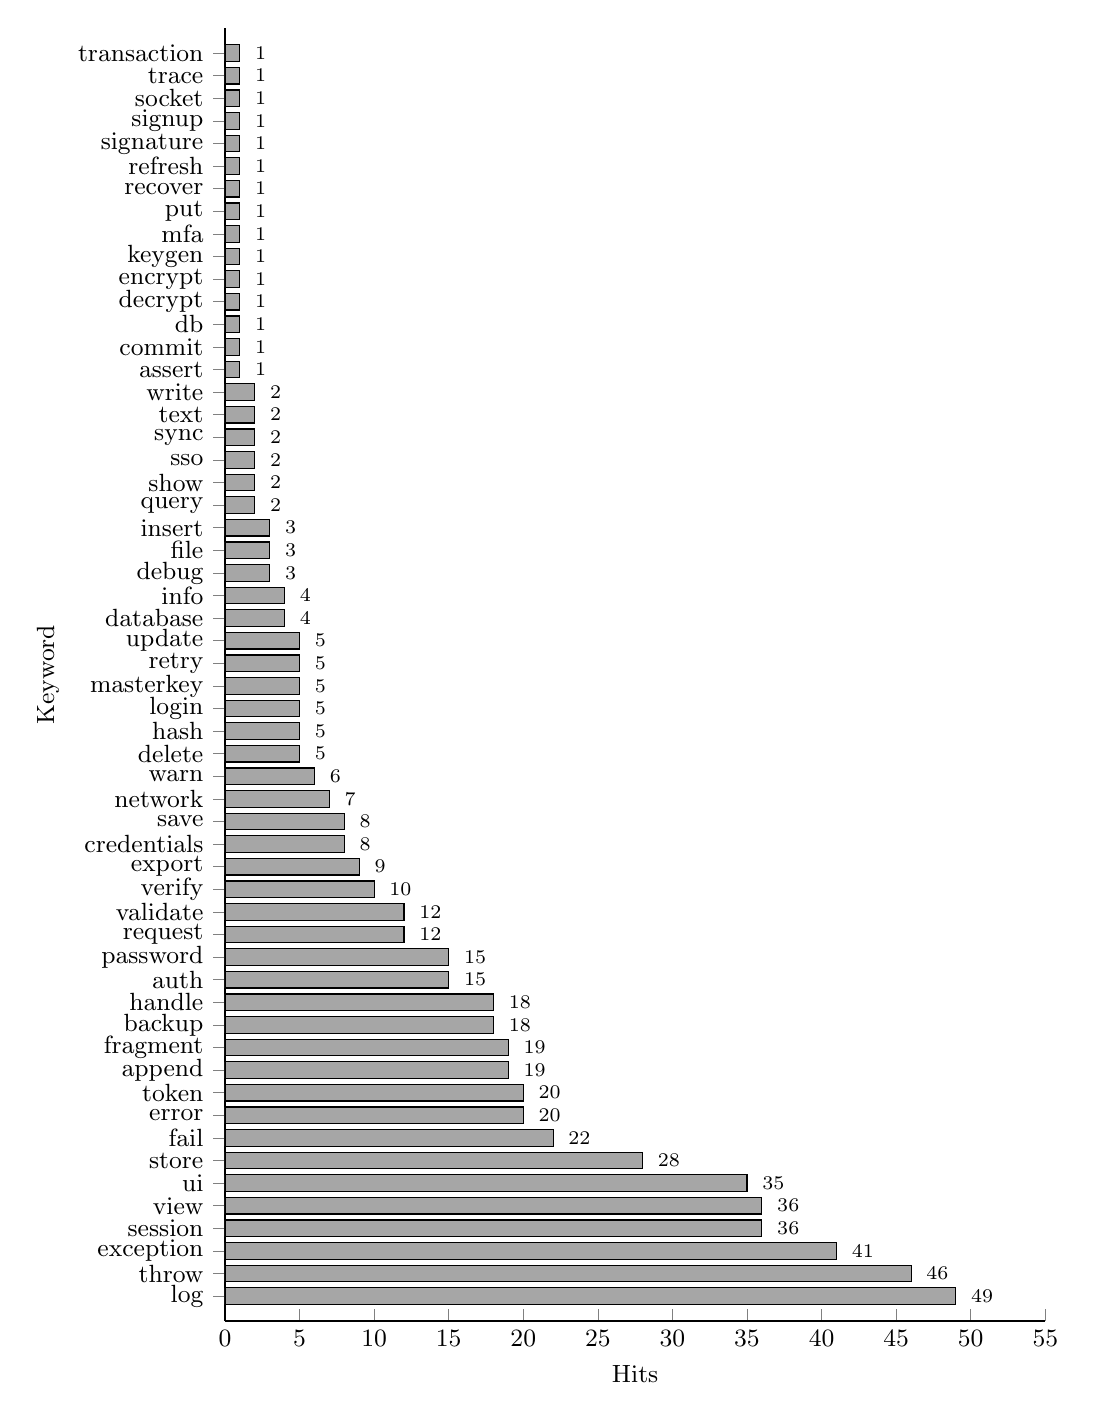
\begin{tikzpicture}
      \begin{axis}[
        width=12cm,
        height=18cm,
        xbar,
        bar width=6pt,
        font=\small,
        symbolic y coords={
            log,throw,exception,session,view,ui,store,fail,error,token,
            append,fragment,backup,handle,auth,password,request,validate,
            verify,export,credentials,save,network,warn,delete,hash,login,
            masterkey,retry,update,database,info,debug,file,insert,query,
            show,sso,sync,text,write,assert,commit,db,decrypt,encrypt,
            keygen,mfa,put,recover,refresh,signature,signup,socket,trace,
            transaction},
        ytick=data,
        tick label style={font=\small},
        enlarge y limits=0.02,
        xlabel={Hits},
        ylabel={Keyword},
        xmin=0, xmax=55,
        nodes near coords,
        every node near coord/.append style={font=\scriptsize,xshift=2pt},
        axis x line*=bottom,
        axis y line*=left
      ]
        \addplot[xbar,fill=gray!70] coordinates {
          (49,log) (46,throw) (41,exception) (36,session) (36,view)
          (35,ui) (28,store) (22,fail) (20,error) (20,token)
          (19,append) (19,fragment) (18,backup) (18,handle)
          (15,auth) (15,password) (12,request) (12,validate)
          (10,verify) (9,export) (8,credentials) (8,save)
          (7,network) (6,warn) (5,delete) (5,hash) (5,login)
          (5,masterkey) (5,retry) (5,update) (4,database)
          (4,info) (3,debug) (3,file) (3,insert) (2,query)
          (2,show) (2,sso) (2,sync) (2,text) (2,write)
          (1,assert) (1,commit) (1,db) (1,decrypt) (1,encrypt)
          (1,keygen) (1,mfa) (1,put) (1,recover) (1,refresh)
          (1,signature) (1,signup) (1,socket) (1,trace)
          (1,transaction)
        };
      \end{axis}
    \end{tikzpicture}
    \caption{All keyword hits generating categorizations in version diff A}
    \label{fig:commonly_used_words_A_full}
\end{figure}

\begin{figure}
    \centering
    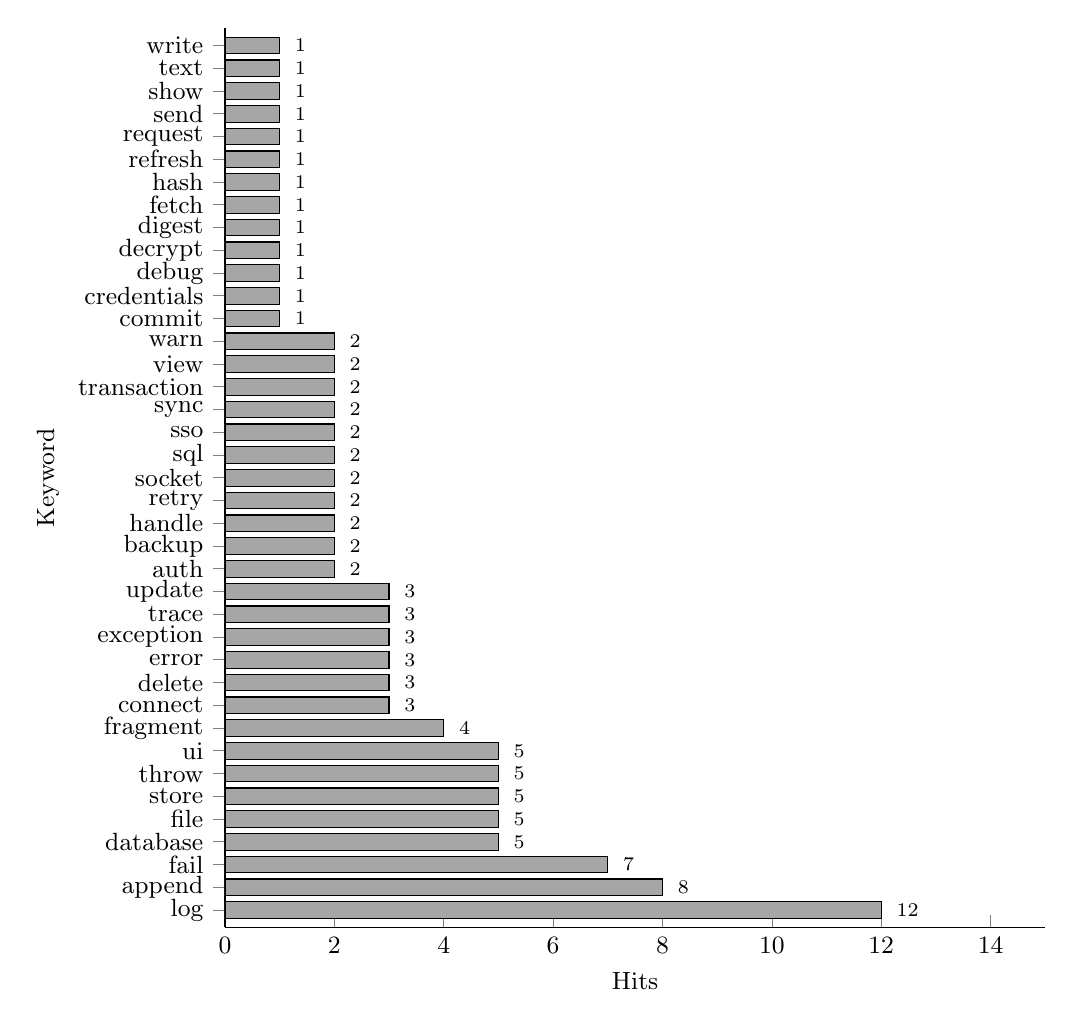
\begin{tikzpicture}
      \begin{axis}[
        width=12cm,
        height=13cm,
        xbar,
        bar width=6pt,
        font=\small,
        symbolic y coords={
            log,append,fail,database,file,store,throw,ui,fragment,connect,
            delete,error,exception,trace,update,auth,backup,handle,retry,
            socket,sql,sso,sync,transaction,view,warn,commit,credentials,
            debug,decrypt,digest,fetch,hash,refresh,request,send,show,text,
            write},
        ytick=data,
        tick label style={font=\small},
        enlarge y limits=0.02,
        xlabel={Hits},
        ylabel={Keyword},
        xmin=0, xmax=15,
        nodes near coords,
        every node near coord/.append style={font=\scriptsize,xshift=2pt},
        axis x line*=bottom,
        axis y line*=left
      ]
        \addplot[xbar,fill=gray!70] coordinates {
          (12,log) (8,append) (7,fail) (5,database) (5,file) (5,store)
          (5,throw) (5,ui) (4,fragment) (3,connect) (3,delete) (3,error)
          (3,exception) (3,trace) (3,update) (2,auth) (2,backup) (2,handle)
          (2,retry) (2,socket) (2,sql) (2,sso) (2,sync) (2,transaction)
          (2,view) (2,warn) (1,commit) (1,credentials) (1,debug) (1,decrypt)
          (1,digest) (1,fetch) (1,hash) (1,refresh) (1,request) (1,send)
          (1,show) (1,text) (1,write)
        };
      \end{axis}
    \end{tikzpicture}
    \caption{All keyword hits generating categorizations in version diff B}
    \label{fig:commonly_used_words_B_full}
\end{figure}

\begin{figure}
    \centering
    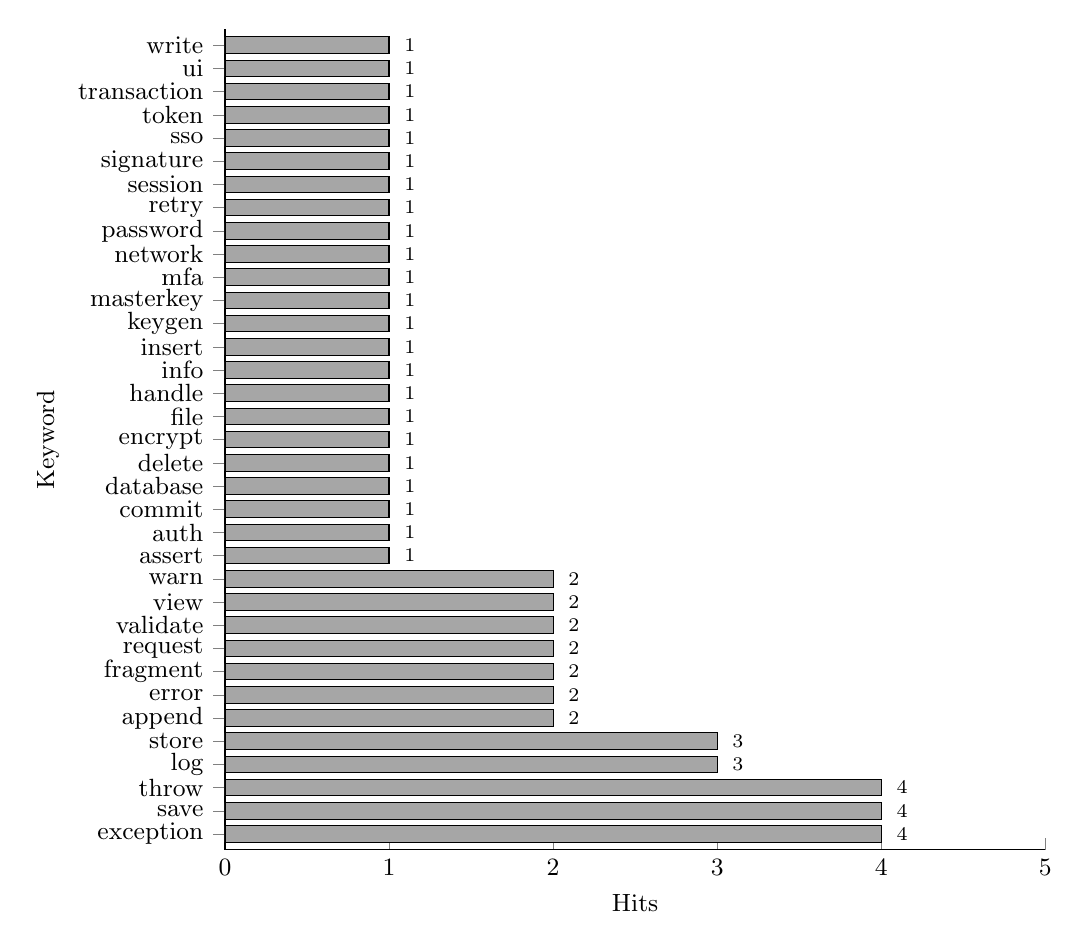
\begin{tikzpicture}
      \begin{axis}[
        width=12cm,
        height=12cm,
        xbar,
        bar width=6pt,
        font=\small,
        symbolic y coords={
          exception,save,throw,log,store,append,error,fragment,request,validate,
          view,warn,assert,auth,commit,database,delete,encrypt,file,handle,info,
          insert,keygen,masterkey,mfa,network,password,retry,session,signature,
          sso,token,transaction,ui,write},
        ytick=data,
        tick label style={font=\small},
        enlarge y limits=0.02,
        xlabel={Hits},
        ylabel={Keyword},
        xmin=0, xmax=5,
        xtick={0,1,2,3,4,5}, % <- force clean integer ticks
        nodes near coords,
        every node near coord/.append style={font=\scriptsize,xshift=2pt},
        axis x line*=bottom,
        axis y line*=left
      ]
        \addplot[xbar,fill=gray!70] coordinates {
          (4,exception) (4,save) (4,throw)
          (3,log) (3,store)
          (2,append) (2,error) (2,fragment) (2,request) (2,validate)
          (2,view) (2,warn)
          (1,assert) (1,auth) (1,commit) (1,database) (1,delete)
          (1,encrypt) (1,file) (1,handle) (1,info) (1,insert) (1,keygen)
          (1,masterkey) (1,mfa) (1,network) (1,password) (1,retry)
          (1,session) (1,signature) (1,sso) (1,token) (1,transaction)
          (1,ui) (1,write)
        };
      \end{axis}
    \end{tikzpicture}
    \caption{All keywords resulting in incorrect categorization for version diff A}
    \label{fig:keyword_incorrect_trigger_A_full}
\end{figure}



\end{appendices}